\chapter{Outlook}
\label{outlook}

In order to finalise the measurement setup Artificial Eye, more development steps will be necessary:
\begin{itemize}
	\item \textbf{Hard metrology:} The mathematic models for surface texture and colour measurements need to be implemented into the software of the Artificial Eye. 
	\item \textbf{Soft metrology:} The scientific study of the human visual perception needs to be conducted and evaluated.
	\item \textbf{Correlation of hard and soft metrology:} The data from both, the optical (hard metrology) setup and the scientific (soft metrology) study need to be correlated. This step is very important and will have a big impact on the final results.
	\item \textbf{Final qualification:} Finally a study needs to be made about the accuracy of the measurements conducted with the Artificial Eye. This will show how precisely the setup can reflect the human visual perception.
\end{itemize}

In figure \ref{ChainOutlook} the remaining development steps are shown as red-bordered, the already finished steps are shown as green-bordered. In the end, the task of the Artificial Eye is to project the subjective human perception of a product onto an objective scale. Therefore, the most important and challenging step in the future will be the correlation of the two research topics of hard and soft metrology. The final qualification will then show if the Artificial Eye will be a tool usable as a device in quality control.

\begin{figure}[h]
\begin{center}
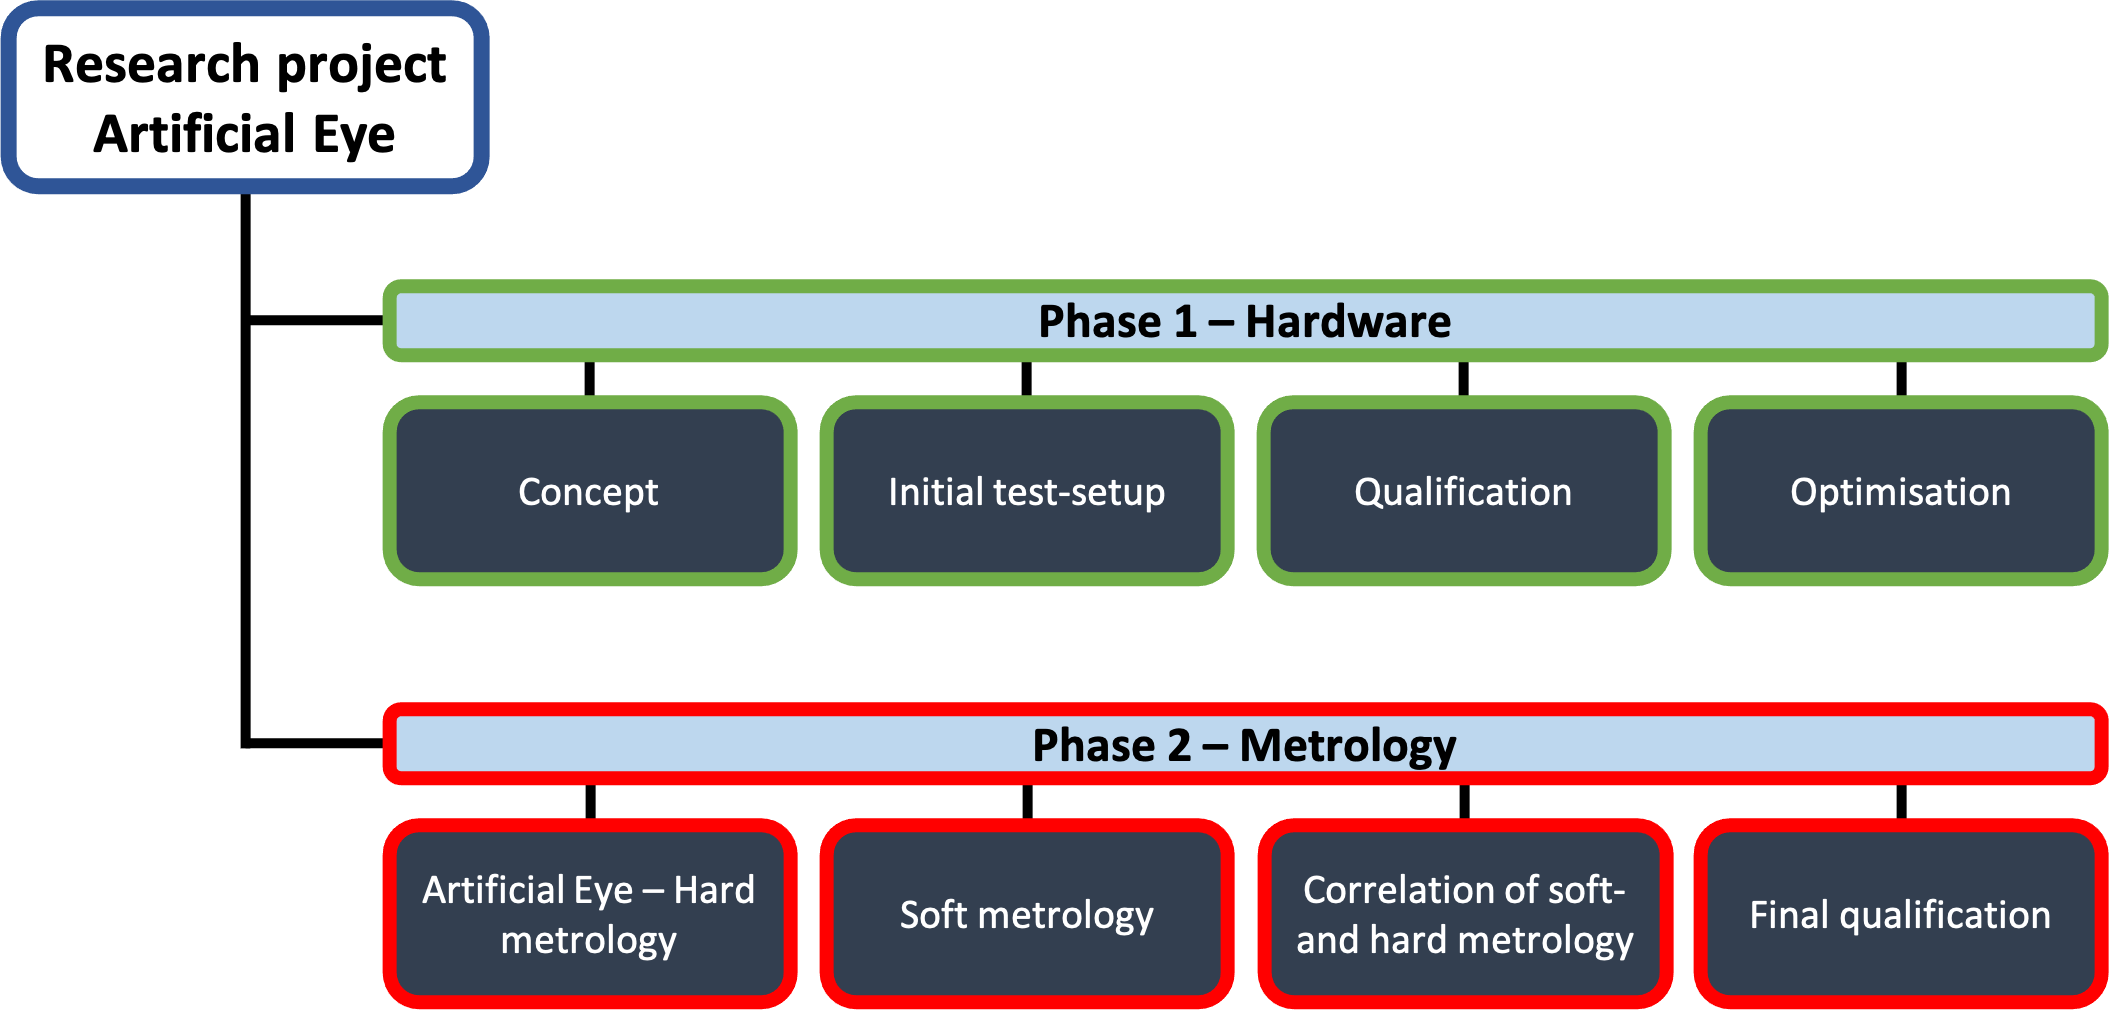
\includegraphics[width=12cm]{Pictures/ChainOutlook}
\caption[Overview of the remaining development steps]{Overview of the remaining development steps: Green - Completed, Red - Open}
\label{ChainOutlook}
\end{center}
\end{figure}